\chapter{Formalizing claims}
\label{chap:formalization}

In the previous chapter we have explored how to identify claims in text. 
Now, we wish to lay the ground work for the next step: structuring those claims. 
To do so, we first need a model according to which the claims will be structured. 
Unlike most approaches in argumentation mining and computational argumentation that
assume a claim is atomic, we wish to work on the sub-claim level in an attempt to 
derive a logical representation of claims. 

% TODO this needs further writing
This chapter is divided into two main parts. 
In the first part, the microstructure formalism is introduced 
(section~\ref{sec:for_microstructures}). 
In the second part, we introduce a
a formalization based on ontologies. 

\section{Microstructures}
\label{sec:for_microstructures}

\begin{figure}
	\begin{center}
      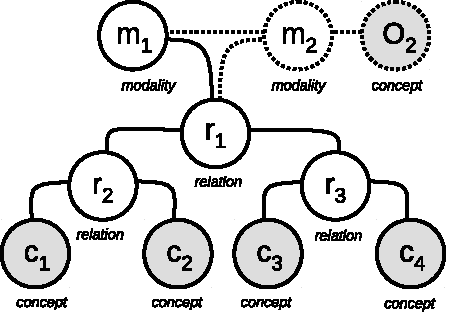
\includegraphics[scale=1]{microstructure.pdf}
      \end{center}
      \caption{Claim microstructure (2nd-order).}
  \label{fig:structures_flowchart}
\end{figure}

Microstructures are structures expressing relations between the domain-specific
concepts, reflecting beliefs, value judgements, or desired policies of the claim
author. Their purpose is to capture the gist of the claim. 
They stemmed from as many claims could be expressed as a \emph{relation}
between \emph{concepts} using a certain \emph{modality}. 
Figure~\ref{fig:structures_flowchart} shows a claim microstructure bringing three elements 
together. 

\paragraph{Relations. }  Many claims can be represented as expressing a
relation between two concepts. For example, on the topic of ``Gay Rights'', 
the relations may be `\texttt{promotes(gay marriage, depopulation)}' and 
`\texttt{purpose(love, procreation)}'. 
There are also comparably fewer claims that can be expressed via
higher-order relations , e.g. `\texttt{entails(constitution, allow(state, gay marriage))}. 
Each relation can be negated, e.g. $\neg$\texttt{promotes(gay marriage,
depopulation)} expresses that gay marriage does not cause depopulation. 
Relations are domain independent. 

\paragraph{Concepts. }
The relations are established between concepts, expressed by noun phrases. 
For ease of access, they can be arranged into a small, domain specific taxonomy of concepts. 
For instance ``gay marriage'', ``heterosexual marriage'' and ``religious marriage''
all belong under the concept of ``marrriage''. 
The taxonomic relations could also be useful for later computational processing. 
Concepts are domain dependent and need to defined for each topic anew

\paragraph{Modalities. }
We observe that claims are expressed under different modalities. 
They can be roughly categorized into \textit{beliefs, value judgements, and policies}. 
We formalize this via unary relations `believes', `approves', `disapproves',
and `desires' corresponding 
to beliefs (factual, religous, and opinion-based), positive value judgements, negative value 
judgements, and desired policy (desired state of affairs) respectively. 
The three modalities act as a wrapper on the propositional content of the claim, 
effectively modulating what is being claimed. 
For instance, `\texttt{believes(purpose(love, procreation))}' expresses the belief 
that love serves procreation, while \texttt{desires(}$\neg$\texttt{allow(state, gay marriage))}'
expresses the wish for the state not to allow gay marriages. 

\paragraph{Second opinion holder. }
Finally, in a number of claims the claim is expressed with a reference to a second
opinion holder (e.g. the Bible, the state). 
To tackle this, we add an additional modality layer with the opinion holder as
an additional modifier. 
For instance `\texttt{believes(believes[state](promotes(marriage, advancement)))}' corresponds
to the belief that the state believes gay marriages lead to an advancement. 
By convention, the opinion holder of the first modality is always the author of the post. 

\begin{table}
{\footnotesize
\begin{tabular}{lp{0.80\columnwidth}}
\toprule
\textbf{Relation} & \textbf{Definition} \\
\midrule
\texttt{promotes(A, B)} & Promoting agent A promotes, fosters, leads, increases likelihood, boosts B.  \\
\texttt{suppress(A, B)} & Suppressing agent A suppresses, decreases likelihood, puts down, vanquishes B \\
\midrule
\texttt{allow(A, B)} & Principle A allows, approves, licenses state of affairs B \\
\midrule
\texttt{entails(A, B)} & State of affairs A, necessarily, per definition or causally, makes B true. \\
\texttt{contradicts(A, B)} & State of affairs A, necessarily, per definition or causally, makes B false. \\
\midrule
\texttt{purpose(A, B)} & The purpose of A is B. \\
\midrule
\texttt{equal(A, B)} & State of affairs A is equal to state of affairs B. \\
\midrule
\texttt{has(A, B)} & A has the properties affected by the existence of B.  \\
\bottomrule
\end{tabular}}
\caption{Relation types in claim microstructures.}
\label{tab:microstructures_relations}
\end{table}

\paragraph{Microstructure formalization. }$\mathcal{R}, \mathcal{C}$, and
$\mathcal{M}$ denote the set of relations, concepts and
modalities, respectively. 
Formally, we define a claim microstructure as a quadruple 
$$
(m_1, m_2, o_2, r)
$$ 
where $m_1 \in \mathcal{M}$, $m_2 \in \mathcal{M} \cup \{\epsilon\}$,
$o_2 \in \mathcal{C} \cup \{\epsilon\}$ is the optional second opinion holder, and 
$r = (t, c_1, c_2) \in \mathcal{R}$ is the (possibly higher order) relation 
between two concepts or relations $c_1, c_2 \in \mathcal{C} \cup \mathcal{R}$
conveyed by the relation type $t$.
Table~\ref{tab:microstructures_relations} lists all possible relation types. 
In chapter~\ref{chap:analysis} we will show
how this microstructure formalization can be used. 
Now that we have formally defined microstructures, we move on to another
formal claim representation. 

\section{Ontology-based formalization}

Microstuctures provide a claim structure which can then be used 
to ``compress'' the claim for subsequent argumentation tasks
(see application to stance classification in section~\ref{sec:stance_micro}).
However, microstructures do not inherently support any
well-established computer science standard. 
Hence, we turn to ontologies. Using ontologies not only allows for 
formalizing a claim, but also provides inference opportunities within
a well-established frameworks (such as the resource description framework RDF). 

We propose an ontology-based framework ClaimOntology to  formalize claims. The
ontology is key part of a formalization framework which defines how to
bootstrap a claim formalization from scratch. The end product of the workflow
is a ontology containing formalized claims in a specific domain. 
The ontology itself is built on two levels: 
\begin{enumerate*}[label=(\arabic*)]
\item the upper and 
\item the domain ontology 
(the motivation of using two-level ontologies is described in
		section~\ref{sec:knowledge_representation}). 
\end{enumerate*}
The upper ontology formalizes abstract patterns in argumentative
claims as object properties. The domain-level ontology conceptualizes 
a specific discussion domain. The relationship between the upper 
and domain ontology is similar to a predicate-argument
relationship \citep{hindle1990noun}, where the upper ontology
defines argumentation-specific predicates --- defined through object properties, 
and the domain ontology defines arguments --- defined through 
individuals. 

The steps to be able to perform domain-specific claim analysis
involve
\begin{enumerate*}[label=(\arabic*)]
\item domain experts designing the domain ontology,
\item integrating the proposed domain ontology with the upper ontology,
\item defining the claims as individuals in the two-level ontology, and
\item validating claim individuals to ensure quality of fit for
	individuals in the domain ontology
\end{enumerate*}
Completing these steps allows users of the formalization framework
to do deep domain claim analysis for the domain of interest. 
An example of a deep domain analysis is in chapter~\ref{chap:analysis}.

Apart from modeling domain concepts and the relationships amongst them, we also
wish to formalize the \emph{modality} of how the claim was expressed: as facts,
policies, and positive or negative value statements (see definition in
\citep{rieke1997argumentation} and microstructure
section~\ref{sec:for_microstructures}). 

\subsection{ClaimOntology}
\label{subsec:claimontology}

The upper ontology represents general argumentation patterns, mostly on the claim level. 
The concepts and relations are used across different domains. 
The central object of the upper ontology is the claim class.
We are interested in extracting as much as possible claims from a single topic. 
We leave the levels above the claim (argument) for future work. The proposed
ontology is an OWL second-order description logic (2DL) ontology built using the
Prot\'{e}g\'{e} software \citep{gennari2003evolution}. The four main concepts of the
upper ontology are:
\begin{itemize}
	\item \texttt{claim}, corresponding to any argumentative statement,
	\item \texttt{speaker},  denoting the author of the claim
		(one speaker may be associated with $N$ \texttt{claims})
	\item \texttt{modality}, which is one of fact, value, or policy, and
	\item \texttt{domain\_topic}, representing any individual from the domain ontology.
\end{itemize}

The main concepts are related to each other through different types of object
properties, suitable to represent both the structural and semantic aspects of
claims. The former aim at formalizing the structure of claims used in
the argumentation, such as the presence of an antecedent element. The latter
are used to describe the semantic relations in claims, for instance that
an element causes another one. Thus, on one hand, the attempt of 
formalizing structural aspects improves the analysis of structuring and
forming process of argumentation. On the other hand, this type of formalization
is allows for a semantic analysis of building blocks, namely claims, used in 
argumentative discussions. Among the structural properties, we identify:
\begin{itemize}
\item \texttt{has\_declaration}, 
\item \texttt{has\_antecedent},
\item \texttt{has\_opinion\_holder}, and
\item \texttt{has\_claim}. 
\end{itemize}



\begin{figure}
	\centering
\begin{tikzpicture}
\path [mindmap, grow cyclic, level 1/.append style={sibling angle=360/13},
concept color=orange!40,
]
node [concept] {domain topic}[clockwise from=0]
	child { node[concept] {religion}}
	child { node [concept]{plant}}
	child { node[concept] {war}}
	child { node[concept] {organization}}
	child { node[concept] {human being}}
	child { node[concept]  {human rights}}
  child {  node[concept] {plant}}
  child {  node[concept] {status behavior}}
  child {  node[concept] {economic cost}}
  child {  node[concept] {drug}}
  child {  node[concept] {crime}}
  child {  node[concept] {science}}
  child {  node[concept] {disease}};
  child {  node[concept] {society effect}};
	
\end{tikzpicture}
\caption{Marijuana legalization domain ontology classes}
\label{fig:marijuana_domain_ontology}
\end{figure}

\begin{figure}
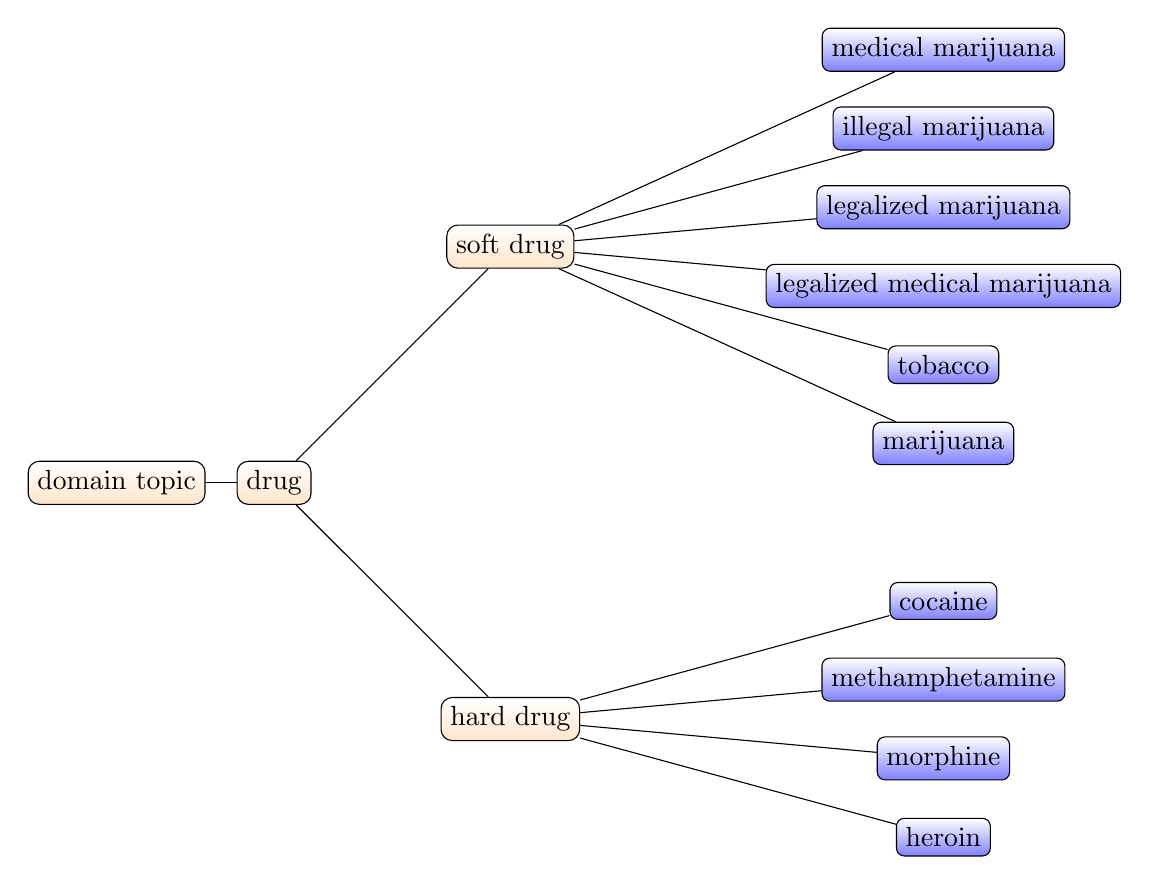
\begin{tikzpicture}
[grow'=right,
level 1/.style={sibling distance=1.5cm, level distance=2cm},
level 2/.style={sibling distance=1.5cm, level distance=3cm, },
level 3/.style={
sibling distance=1cm, level distance=5.5cm},
concept/.style=
{shape=rectangle, rounded corners,
draw, align=center,
top color=white, bottom color=orange!20},
individual/.style={rectangle, rounded corners=1mm, draw, top color=white, bottom color=blue!50,
text centered}
	]
	\node (root) [concept] {domain topic}
	child  { node [concept] {drug}
	child  { node [concept] {soft drug} 
	child { node [individual] {medical marijuana}}
	child { node [individual] {illegal marijuana}}
	child { node [individual] {legalized marijuana}}
	child { node [individual] {legalized  medical marijuana}}
	child { node [individual] {tobacco}}
	child { node [individual] {marijuana}}
    }
    child [missing]
    child [missing]
    child [missing]
    child {node  [concept]{hard drug}
	child {node [individual] {cocaine}}
	child {node [individual] {methamphetamine}}
	child {node [individual] {morphine}}
	child {node [individual] {heroin}}
    }
};
	
\end{tikzpicture}
\caption{Marijuana legalization domain ontology drug individuals. 
	Classes/entities and orange and individuals are blue. }
	\label{fig:drug_domain_individuals}
\end{figure}

\begin{figure}
\begin{tikzpicture}
\end{tikzpicture}
\end{figure}


\begin{figure}
	\centering
	\footnotesize
	\begin{tikzpicture}[
concept/.style={shape=rectangle, rounded corners,
draw, align=center,
top color=white, bottom color=orange!20},
node distance=5cm,
]
\node [concept] (human) {human being};
\node [concept, below right of=human] (domain) {domain topic};
\node [concept, above left of=human] (disease) {disease};
\node [concept, below left of=human] (status) {status behavior};
\node [concept, above right of=human] (drug) {drug};

\draw[densely dashed, color=olive] (human) -- (domain);
\draw[densely dashed, color=olive] (disease) .. controls ($(human) + (-1.3cm, -1.3cm)$) .. (domain); 
\draw[densely dashed, color=olive] (status) -- (domain); 
\draw[densely dashed, color=olive] (drug) -- (domain); 
\draw[densely dashed, color=olive] (human) -- (domain); 

		\draw [->] (human.north) .. controls ($(human.north) + (0cm,
		3cm)$) ..  (drug) node [sloped, above, near end] {buys drugs}; 
		\draw [->] (human.north) .. controls ($(human) + (3.5cm, 1cm)$)
		..  (drug) node [sloped, above, near start] {consumes drugs}; 
		\draw [->] (human) -- (status) node [below, midway, sloped] {has behavior}; 
		\draw [->] (human) -- (disease) node [below, midway, sloped] {has disease}; 
\end{tikzpicture}
	\caption{Dashed lines indicate subclass, full lines indicate object property relations. 
	The triple (\texttt{human\_being}, \texttt{buys\_drugs}, \texttt{drug}) represents an 
	individual that belongs to the
	\texttt{human\_being} class, which posses the property \texttt{buys\_drugs} with 
	object \texttt{drug}.} 
	\label{fig:main-classes}
\end{figure}
